% Options for packages loaded elsewhere
\PassOptionsToPackage{unicode}{hyperref}
\PassOptionsToPackage{hyphens}{url}
%
\documentclass[
]{article}
\usepackage{amsmath,amssymb}
\usepackage{lmodern}
\usepackage{iftex}
\ifPDFTeX
  \usepackage[T1]{fontenc}
  \usepackage[utf8]{inputenc}
  \usepackage{textcomp} % provide euro and other symbols
\else % if luatex or xetex
  \usepackage{unicode-math}
  \defaultfontfeatures{Scale=MatchLowercase}
  \defaultfontfeatures[\rmfamily]{Ligatures=TeX,Scale=1}
\fi
% Use upquote if available, for straight quotes in verbatim environments
\IfFileExists{upquote.sty}{\usepackage{upquote}}{}
\IfFileExists{microtype.sty}{% use microtype if available
  \usepackage[]{microtype}
  \UseMicrotypeSet[protrusion]{basicmath} % disable protrusion for tt fonts
}{}
\makeatletter
\@ifundefined{KOMAClassName}{% if non-KOMA class
  \IfFileExists{parskip.sty}{%
    \usepackage{parskip}
  }{% else
    \setlength{\parindent}{0pt}
    \setlength{\parskip}{6pt plus 2pt minus 1pt}}
}{% if KOMA class
  \KOMAoptions{parskip=half}}
\makeatother
\usepackage{xcolor}
\usepackage[margin=1in]{geometry}
\usepackage{graphicx}
\makeatletter
\def\maxwidth{\ifdim\Gin@nat@width>\linewidth\linewidth\else\Gin@nat@width\fi}
\def\maxheight{\ifdim\Gin@nat@height>\textheight\textheight\else\Gin@nat@height\fi}
\makeatother
% Scale images if necessary, so that they will not overflow the page
% margins by default, and it is still possible to overwrite the defaults
% using explicit options in \includegraphics[width, height, ...]{}
\setkeys{Gin}{width=\maxwidth,height=\maxheight,keepaspectratio}
% Set default figure placement to htbp
\makeatletter
\def\fps@figure{htbp}
\makeatother
\setlength{\emergencystretch}{3em} % prevent overfull lines
\providecommand{\tightlist}{%
  \setlength{\itemsep}{0pt}\setlength{\parskip}{0pt}}
\setcounter{secnumdepth}{-\maxdimen} % remove section numbering
\ifLuaTeX
  \usepackage{selnolig}  % disable illegal ligatures
\fi
\IfFileExists{bookmark.sty}{\usepackage{bookmark}}{\usepackage{hyperref}}
\IfFileExists{xurl.sty}{\usepackage{xurl}}{} % add URL line breaks if available
\urlstyle{same} % disable monospaced font for URLs
\hypersetup{
  pdftitle={Comparision of Covid-19 confirmed and death cases between the US and China},
  pdfauthor={Jiawen Chen},
  hidelinks,
  pdfcreator={LaTeX via pandoc}}

\title{Comparision of Covid-19 confirmed and death cases between the US
and China}
\author{Jiawen Chen}
\date{2022-12-07}

\begin{document}
\maketitle

This is my PM566 Final Project website.

\hypertarget{backgroud-story-introduction}{%
\section{1.Backgroud story \&
Introduction}\label{backgroud-story-introduction}}

I was in the US at the beginning of 2020, and then back to China in
March 2020 and quarentined. So I observed how did the pandemic spreaded
so quickly and sharply increased around the world and specificly in the
US. On the other side, after the few first months in 2020, the pandemic
was considered as well controlled. Therefore, in this project, firstly I
will briefly check through the overall COVID-19 situation in the world
wide. Then I analyzed China and the US seperatly to see the trend. The
final step is to compare with those two countries in terms of confirmed
and deaths number.

\hypertarget{methodsinclude-how-and-where-the-data-were-acquired-how-you-cleaned-and-wrangled-the-data-what-tools-you-used-for-data-exploration}{%
\section{2.Methods:(include how and where the data were acquired, how
you cleaned and wrangled the data, what tools you used for data
exploration)}\label{methodsinclude-how-and-where-the-data-were-acquired-how-you-cleaned-and-wrangled-the-data-what-tools-you-used-for-data-exploration}}

\hypertarget{about-the-data}{%
\subsection{About the data}\label{about-the-data}}

I downloaded the datasets from
``\url{https://data.humdata.org/dataset/novel-coronavirus-2019-ncov-cases}?''in
CSV format and updated daily and then chose the global confirmed and
deaths throughout the whole pandemic (1/22/20-recent two days). The
datas are updated everyday by John Hopkins center.

\hypertarget{preparation}{%
\subsection{Preparation}\label{preparation}}

However, the format of two datasets are about the accumulated-confirmed
and death cases of different countries. So I did some filter out steps
of countries/regions, cleaned and normalized that data, for example
tidying dates and consolidating them into normalized time series. We
have variables called ``province'' ````Country/Region'', ``dates'' and
Lat'' and ``Long'' representing different regions. Notice that each
day's count are in separate columns. For this analysis, it would be
nicer to have a column for date and a column for count instead. Also I
select and transformed these two countries from the total death dataset
into data frames.

\begin{center}\rule{0.5\linewidth}{0.5pt}\end{center}

We have variables called ``province'' ````Country/Region'', ``Lat'',
``Long'' and different dates

\hypertarget{here-it-shows-how-the-confirmed-cases-spread-in-the-world-wide}{%
\section{3. Here it shows how the confirmed cases spread in the world
wide}\label{here-it-shows-how-the-confirmed-cases-spread-in-the-world-wide}}

\begin{verbatim}
##   Province.State Country.Region       Lat     Long sumconfirmed
## 1           <NA>    Afghanistan  33.93911 67.70995       206331
## 2           <NA>        Albania  41.15330 20.16830       333455
## 3           <NA>        Algeria  28.03390  1.65960       271122
## 4           <NA>        Andorra  42.50630  1.52180        47219
## 5           <NA>         Angola -11.20270 17.87390       104750
## 6           <NA>     Antarctica -71.94990 23.34700           11
\end{verbatim}

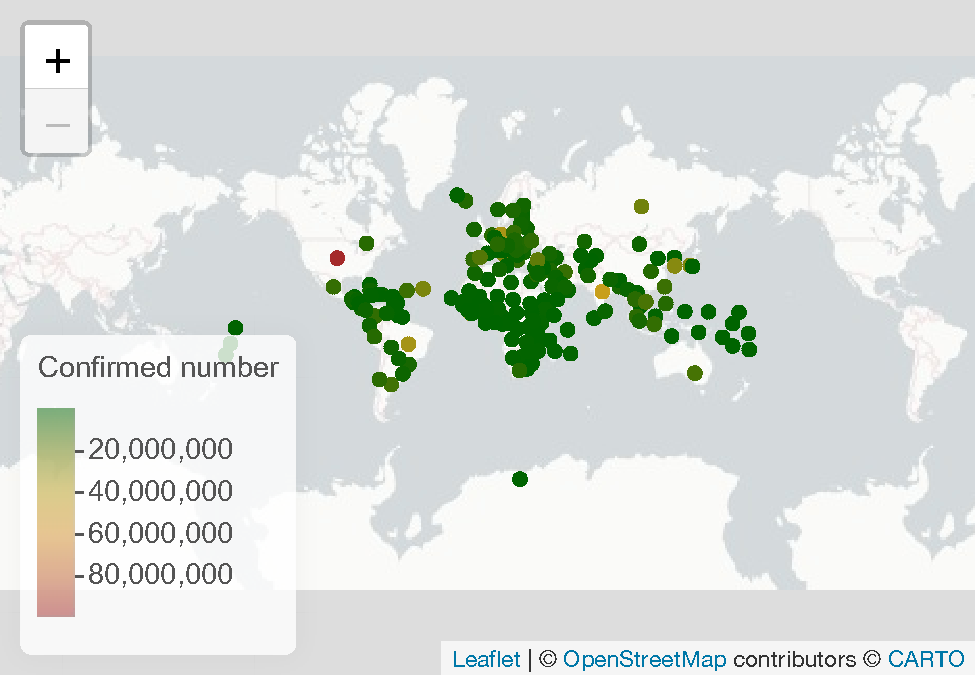
\includegraphics{index_files/figure-latex/unnamed-chunk-2-1.pdf}

From the map, the legend shows the range of confirmed number. The red
color means higher confirmed number. We can see that there America has
the red dot, then India, Brazil and Germany have yellow dots. However,
one drawback of this dataset is that some country, for example China's
data is updated by Province, but the data from the US as a country
total.

\hypertarget{table-to-check-total-confirmed-cases-for-each-country}{%
\section{4. Table to check total confirmed cases for each
country}\label{table-to-check-total-confirmed-cases-for-each-country}}

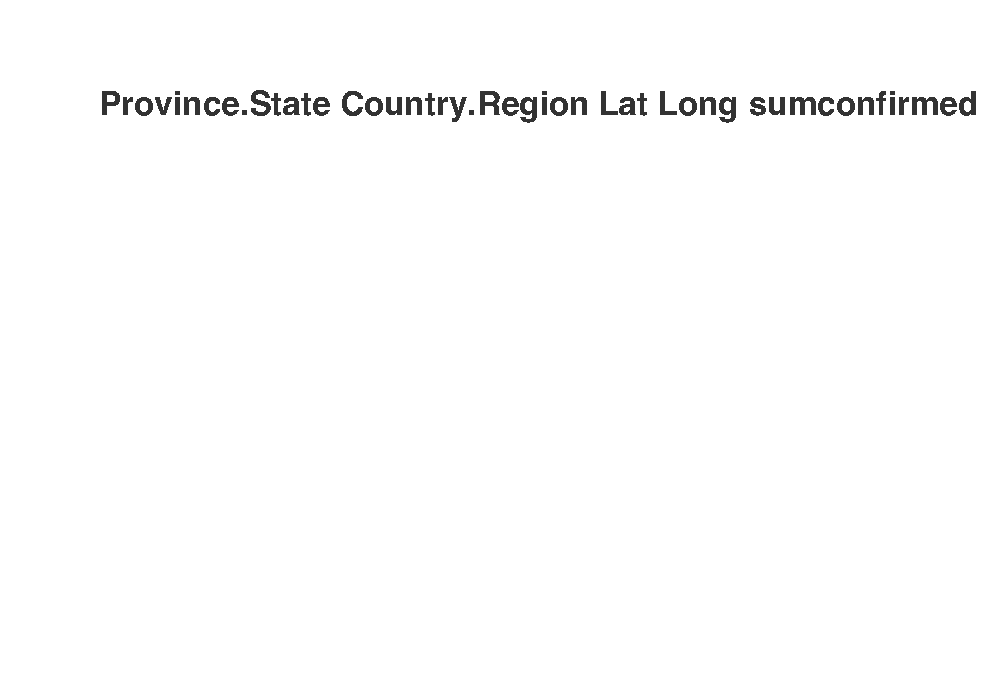
\includegraphics{index_files/figure-latex/unnamed-chunk-3-1.pdf} We can
also check and sort which are the top countries have the greatest or
smallest cases number. Corresponding with the previous heat map, the top
five countries have the greatest cases number are US, India and France
and Germany

\hypertarget{transform-the-total-death-dataset-confirmed-and-deaths-data-of-these-two-countries-into-dataframes}{%
\section{5. Transform the total death dataset, confirmed and deaths data
of these two countries into
dataframes}\label{transform-the-total-death-dataset-confirmed-and-deaths-data-of-these-two-countries-into-dataframes}}

\hypertarget{graphs-of-each-province-in-china-and-us-confirmed-and-deaths-cases.}{%
\section{6.graphs of each province in china and US confirmed and deaths
cases.}\label{graphs-of-each-province-in-china-and-us-confirmed-and-deaths-cases.}}

As I mentioned above, we only have the whole US data, so I just present
the US as a country total. China has 50+ provinces in total and thus can
be hard to represent them all, so I choose the top 6 provinces that have
the largest number of confirmed cases. For the death cases, I only
choose the provinces have more than 1000 death cases.

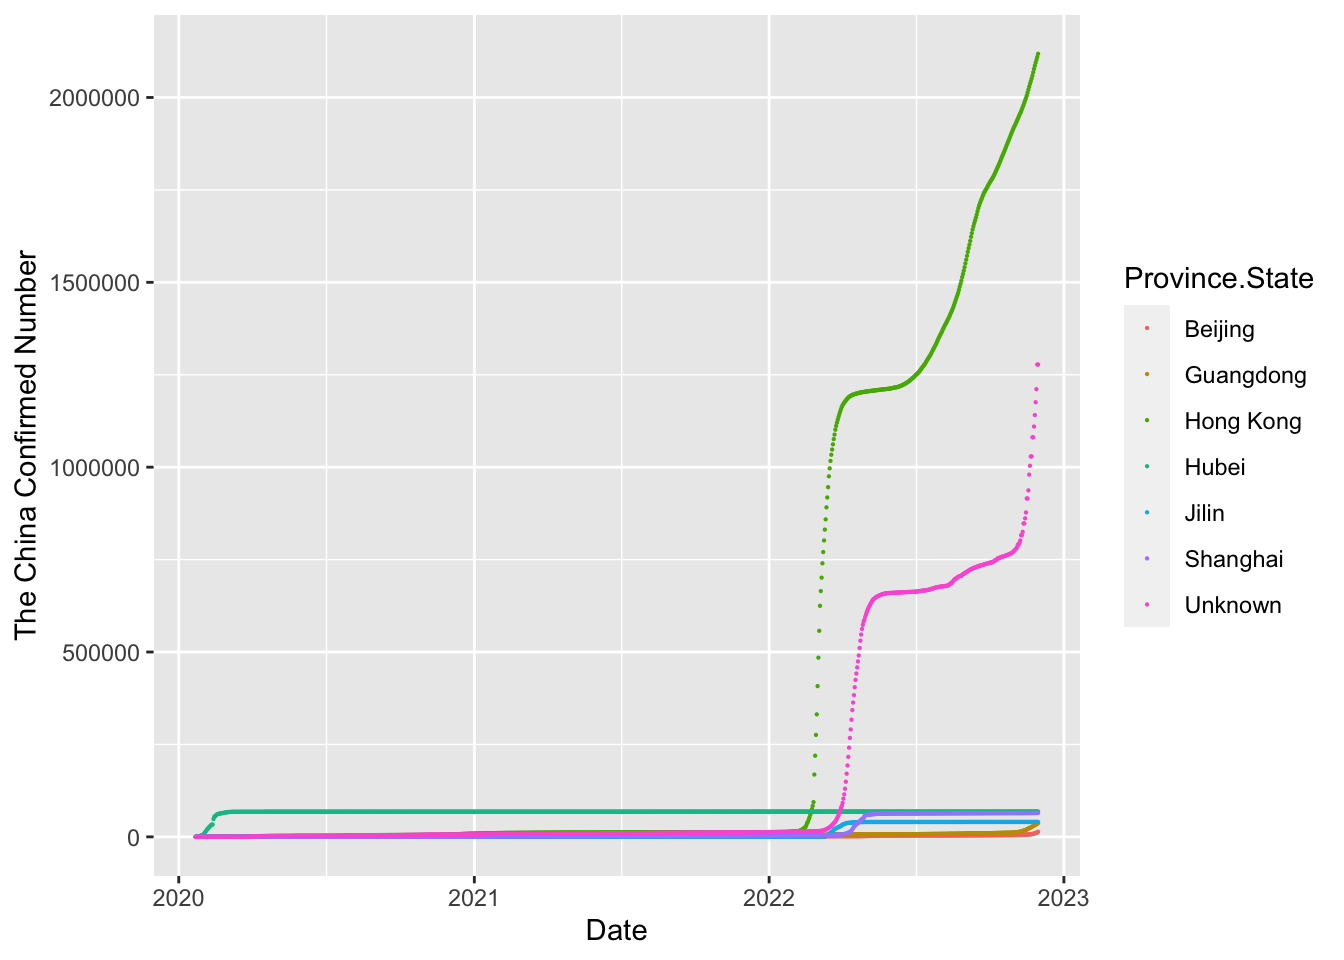
\includegraphics{index_files/figure-latex/unnamed-chunk-5-1.pdf}
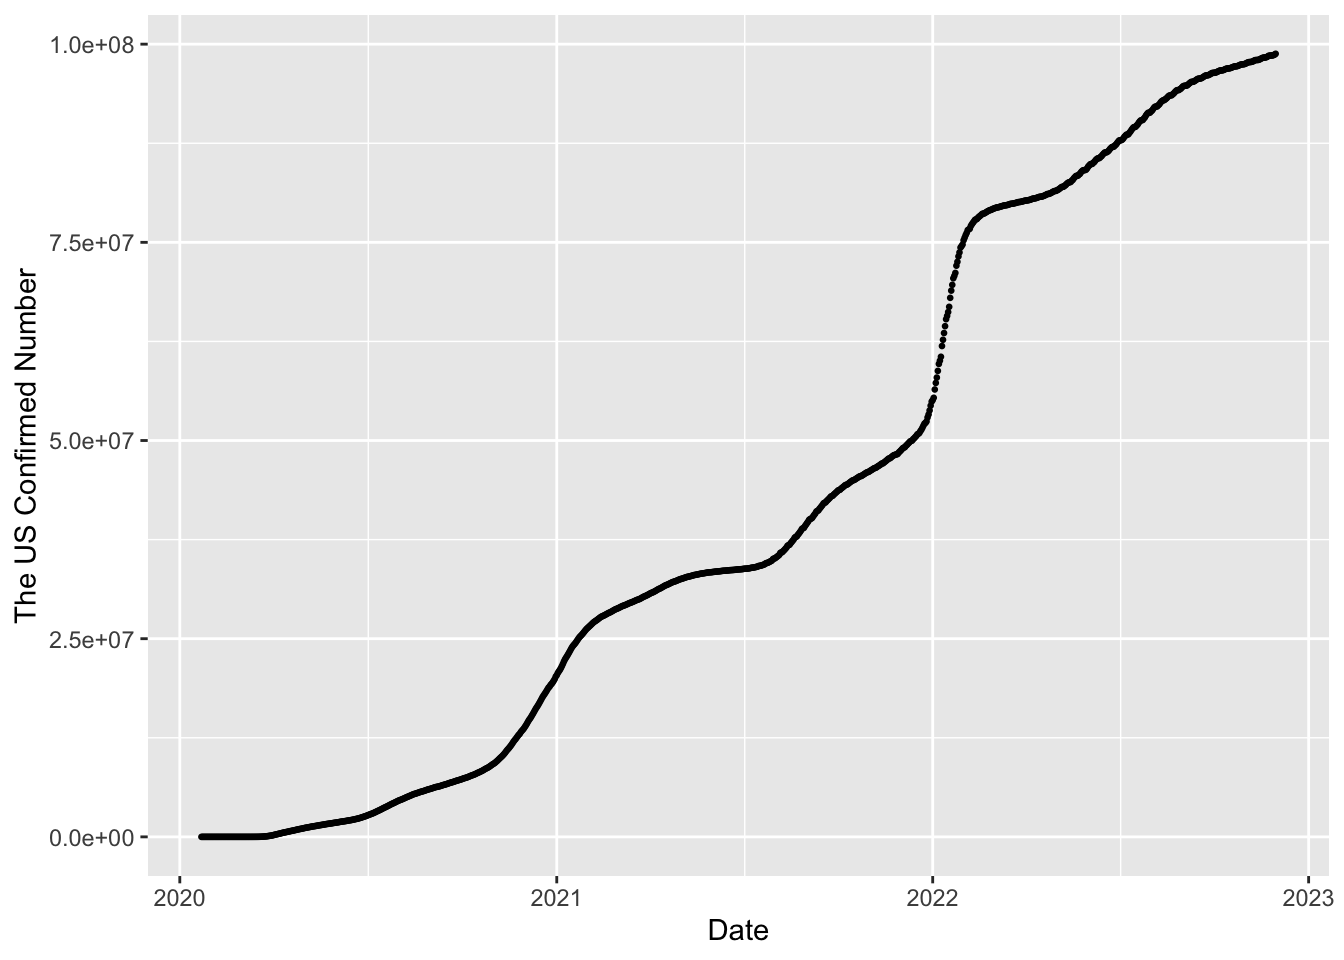
\includegraphics{index_files/figure-latex/unnamed-chunk-5-2.pdf}
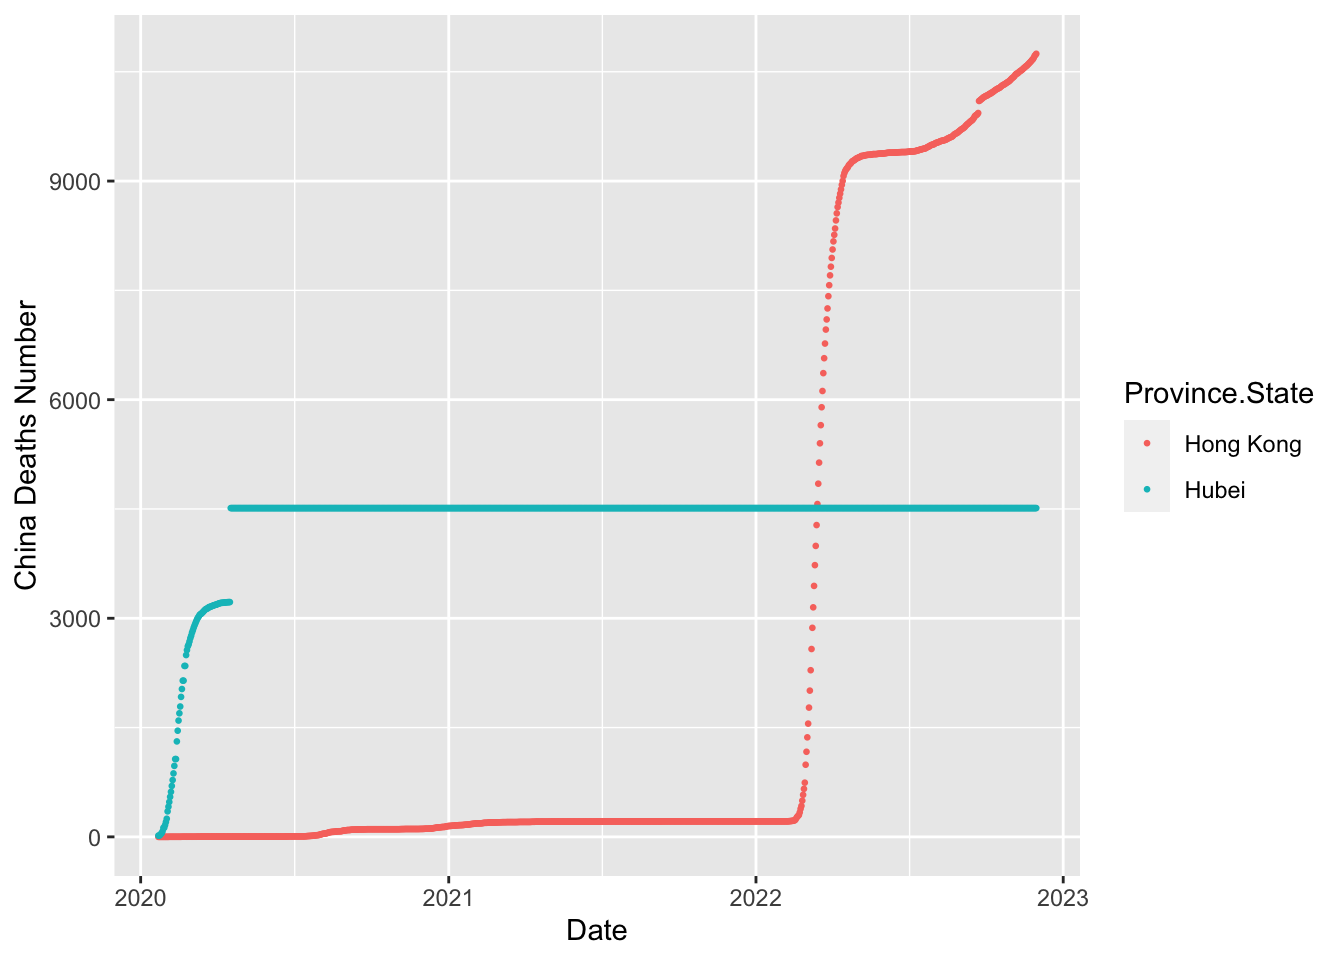
\includegraphics{index_files/figure-latex/unnamed-chunk-5-3.pdf}
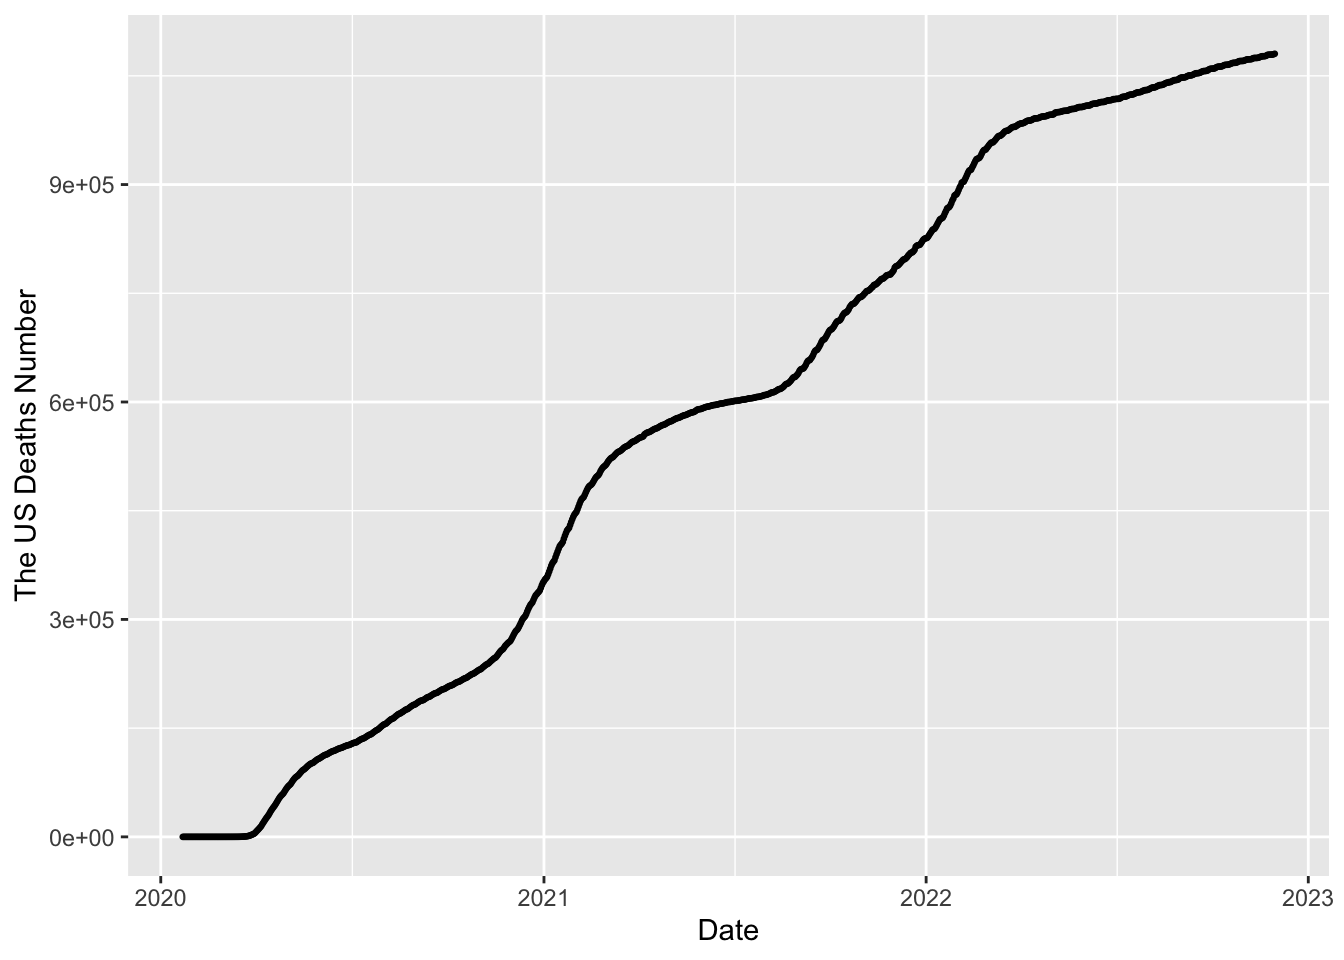
\includegraphics{index_files/figure-latex/unnamed-chunk-5-4.pdf} The top
6 provinces/region that have the largest number confirmed case are
Hongkong, Hubei, Shanghai, Jilin, Guangdong and Beijing. Hongkong is the
city with the most COVID-19 confirmed cases according to the graphs, and
it is the only region with more than 5000 death cases.

\hypertarget{lets-make-those-two-contries-in-comparision}{%
\section{7. let's make those two contries in
comparision}\label{lets-make-those-two-contries-in-comparision}}

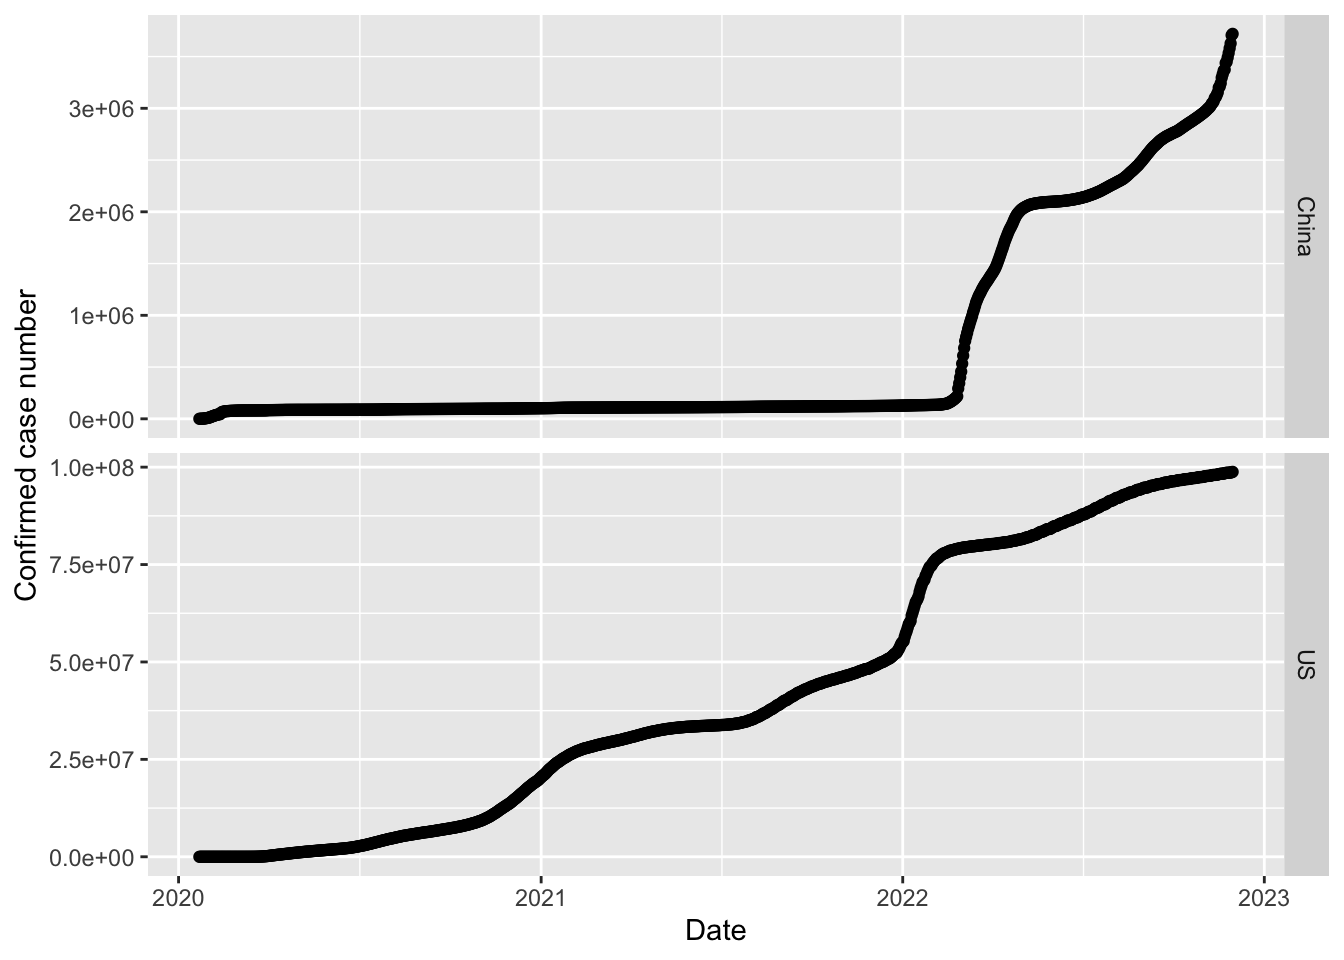
\includegraphics{index_files/figure-latex/unnamed-chunk-6-1.pdf}
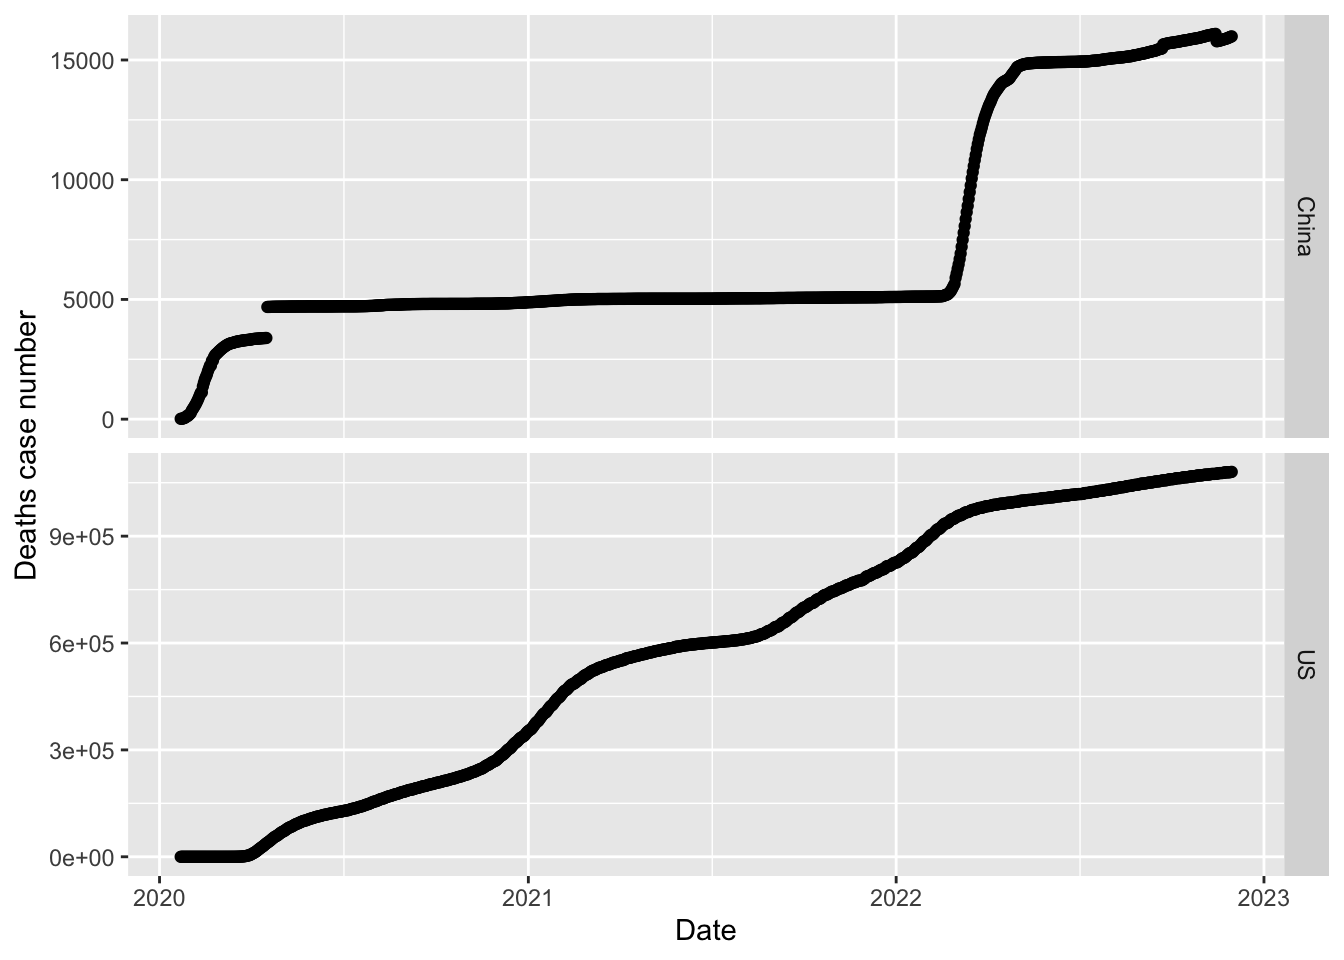
\includegraphics{index_files/figure-latex/unnamed-chunk-6-2.pdf}

\begin{center}\rule{0.5\linewidth}{0.5pt}\end{center}

\hypertarget{conclusion-and-summary}{%
\section{Conclusion and Summary}\label{conclusion-and-summary}}

We can see China started confirming cases ealier than the US but the
confirmed and deaths cases increased slightly until the beginning of
2022. However, the overall confirmed and deaths cases in the US (Until
11/29/2022, deaths cases is 1.09M, from Wikipedia) are significantly
higher than China (until 11/29/2022 deaths cases is 5233, from
Wikipedia). Part of the reason is probably because of the strict
COVID-19 policies. In terms of Hongkong, it executed different policies
compared with the mainland of China

\end{document}
